\documentclass{beamer}
\usetheme[
    numbering=none,
    progressbar=head,
]{metropolis}

\usepackage{graphicx}
\graphicspath{ {../images/} }

\usepackage{amsmath}

\title{On Parameterized Vertex Cover in Streaming}
\date{July 6, 2020}
\author{Adam Cox}
\institute{
    School of Computer Science \\
    University of Birmingham
}

\begin{document}

\maketitle

\begin{frame}{Graph Theory}
    \begin{columns}
        \begin{column}{0.55\textwidth}
            \begin{block}{Nodes/Vertices}
                Representing objects
            \end{block}
            \begin{block}{Edges}
                Representing relationships between objects
            \end{block}
        \end{column}
        \begin{column}{0.35\textwidth}
            \begin{center}
                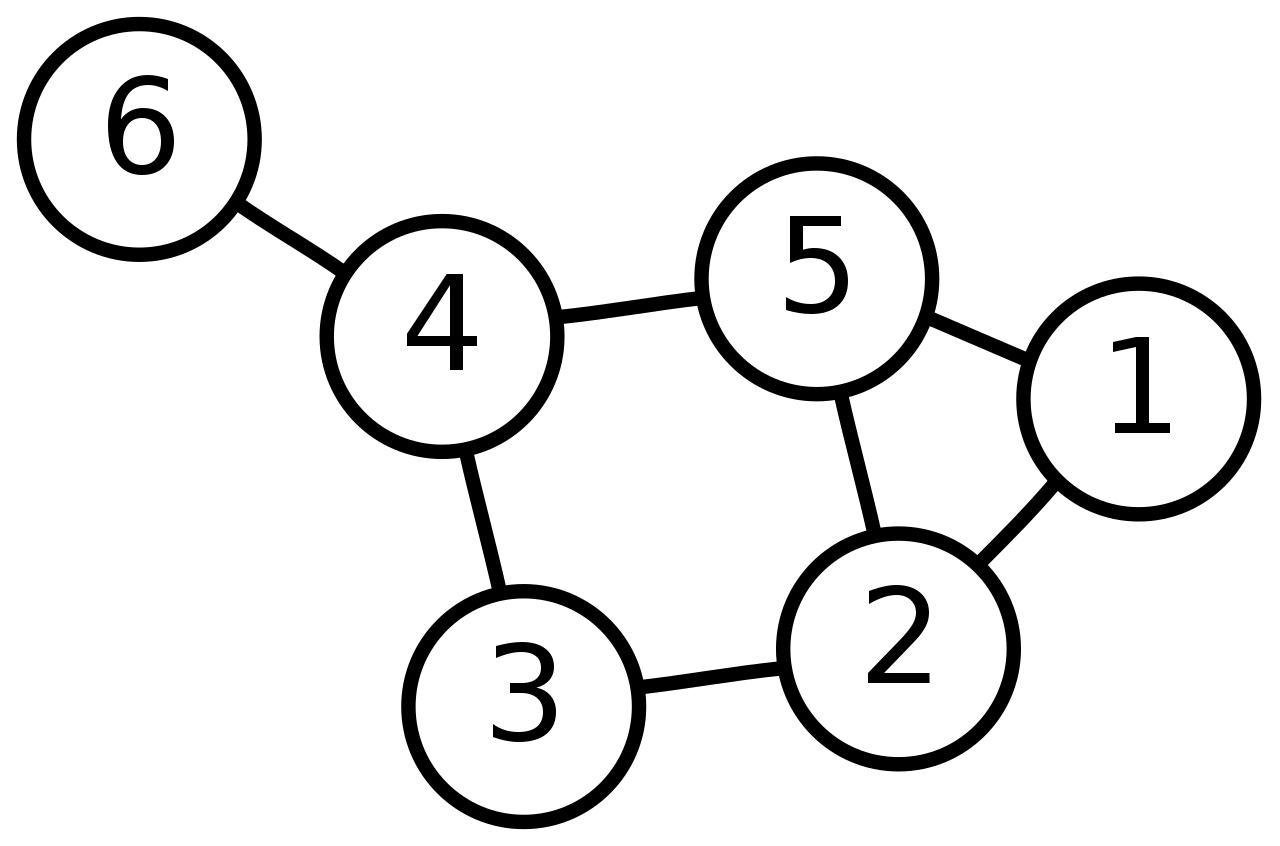
\includegraphics[width=\textwidth]{graph-theory}
            \end{center}
        \end{column}
    \end{columns}

    \begin{center}
        Together this makes a \textbf{graph}
    \end{center}
\end{frame}

\begin{frame}{Vertex Cover}
    \begin{columns}
        \begin{column}{0.6\textwidth}
            A set of vertices that includes at least one endpoint of every edge of the graph.

            \hfill

            A real life example would be putting up cameras at road intersections to be able to see down every road.
        \end{column}
        \begin{column}{0.3\textwidth}
            \begin{center}
                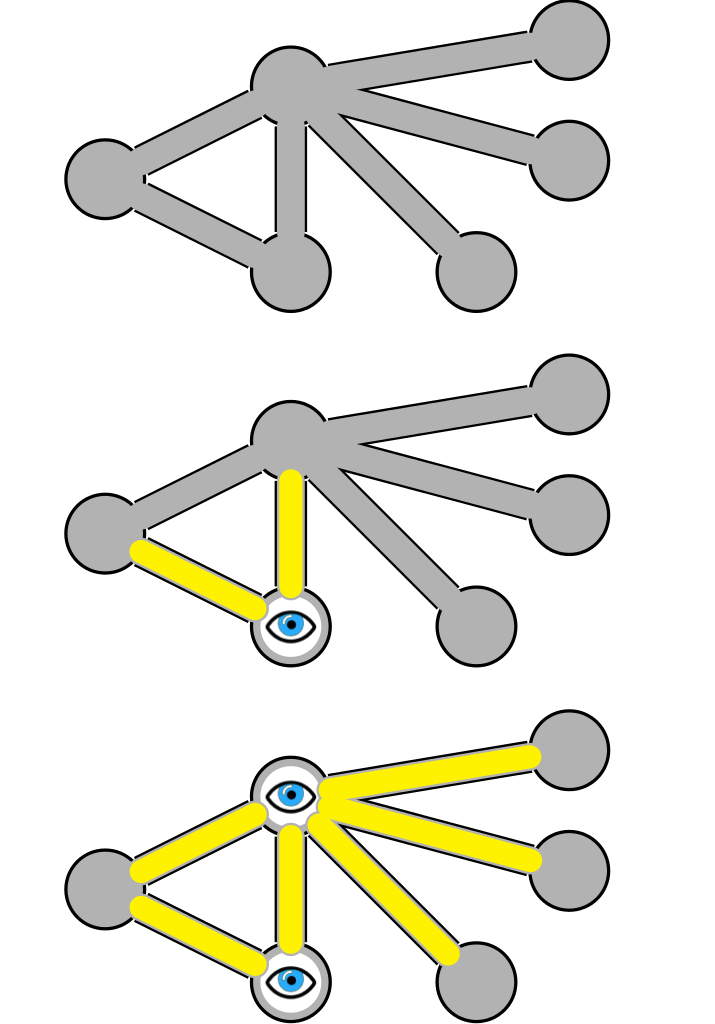
\includegraphics[width=\textwidth]{vertex-cover}
            \end{center}
        \end{column}
    \end{columns}
\end{frame}

\begin{frame}{Karp's 21 NP-complete problems}
    The vertex cover problem is an NP-complete problem: it was one of Karp's 21 NP-complete problems.

    It is often used in computational complexity theory as a starting point for NP-hardness proofs.
\end{frame}

\begin{frame}{Parameterized Algorithms}
    Classical complexity measures runtime of an algorithm solely based on the input size.

    Parameterized complexity measures runtime of an algorithm based on parameters of the input or output.

    \hfill

    Non-parameterized/classical time complexity has been used since the 1960s. Parameterized time complexity only came about in the 1990s.
\end{frame}

\begin{frame}{Parameterized Vertex Cover}
    This is known as the \textbf{Vertex Cover Problem} or k-VC

    \hfill

    \begin{alertblock}{k-VC}
        INSTANCE: Graph $G$ and positive integer $k$\\
        QUESTION: Does $G$ have a vertex cover of size at most $k$?\\
    \end{alertblock}

    \hfill

    The vertex cover problem is an NP-complete problem
\end{frame}

\begin{frame}{Big Data and Streaming}
    Big Data applies to any dataset that is too big to store/look at in one go. We need other methods to be able to make the data usable.

    \hfill

    Non-parameterized space complexity began being studied around the 2000s and only in 2014 did parameterized space complexity start being covered.
\end{frame}

\begin{frame}{Parameterized Vertex Cover in Streaming}
    So for the full problem, we are looking at:

    \begin{itemize}
        \item Insertion-only stream of edges
        \item Value $k$
    \end{itemize}

    And we want a True/False answer. In practise, users would also want the set of vertices that make up the vertex cover.
\end{frame}

\begin{frame}{Historically}
    \begin{block}{}
        \begin{columns}
            \begin{column}{0.45\textwidth}
                \textbf{Branching}

                \begin{itemize}
                    \item Easy logarithmic complexity
                    \item Simple implementation
                \end{itemize}
            \end{column}
            \begin{column}{0.45\textwidth}
                \textbf{Kernelization}

                \begin{itemize}
                    \item Simple rules
                    \item Powerful if done right
                \end{itemize}
            \end{column}
        \end{columns}
    \end{block}
\end{frame}

\begin{frame}{State of the Art}
    In 2014, Chitnis et al put forward streaming algorithms based on these two ideas.

    Branching - Space required is $O(k \boldsymbol\cdot \log n)$ and requires $2^k$ passes

    Kernel - Space required is $O(k^2)$ and requires 1 pass
\end{frame}

\begin{frame}{Implementation}
    So I built these streaming algorithms into a number of domains:

    \begin{itemize}
        \item Local
        \item Local-Stream
        \item Stream
    \end{itemize}
\end{frame}

\begin{frame}{\alert{Local} - Visualisation}
    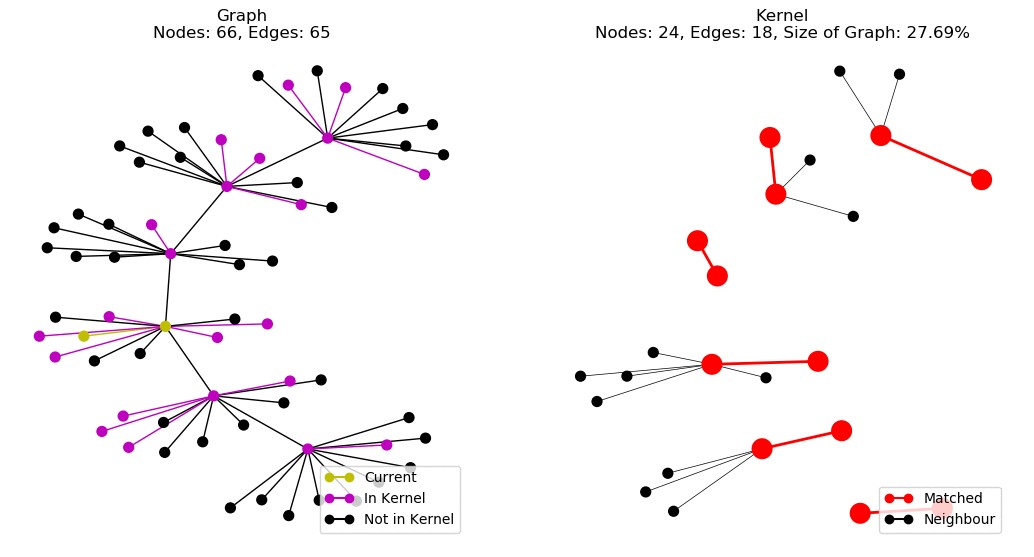
\includegraphics[width=\textwidth]{demo_kernel.jpg}
\end{frame}

\begin{frame}{\alert{Local-Stream} - Performance Profiling}
    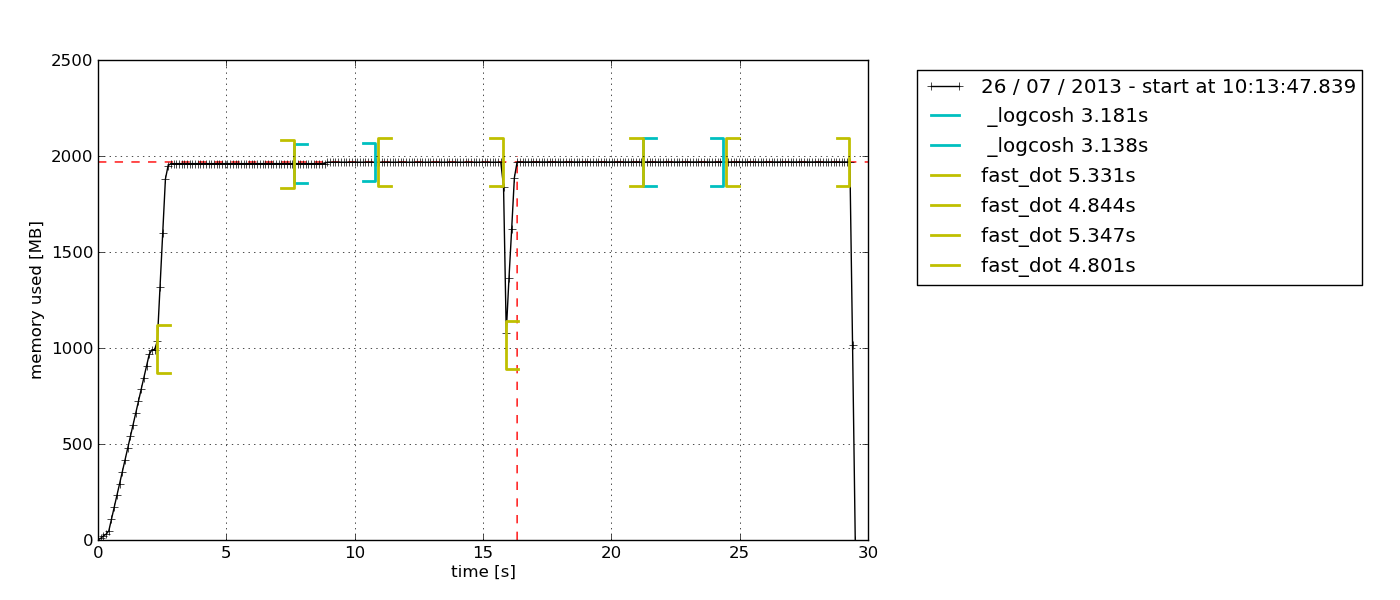
\includegraphics[width=\textwidth]{memory-profiler}

    \hfill

    Disclaimer: This is just an example of what a memory profiling graph looks like.
\end{frame}

\begin{frame}{\alert{Stream} - Graph Streaming Platform}
    \begin{columns}
        \begin{column}{0.7\textwidth}
            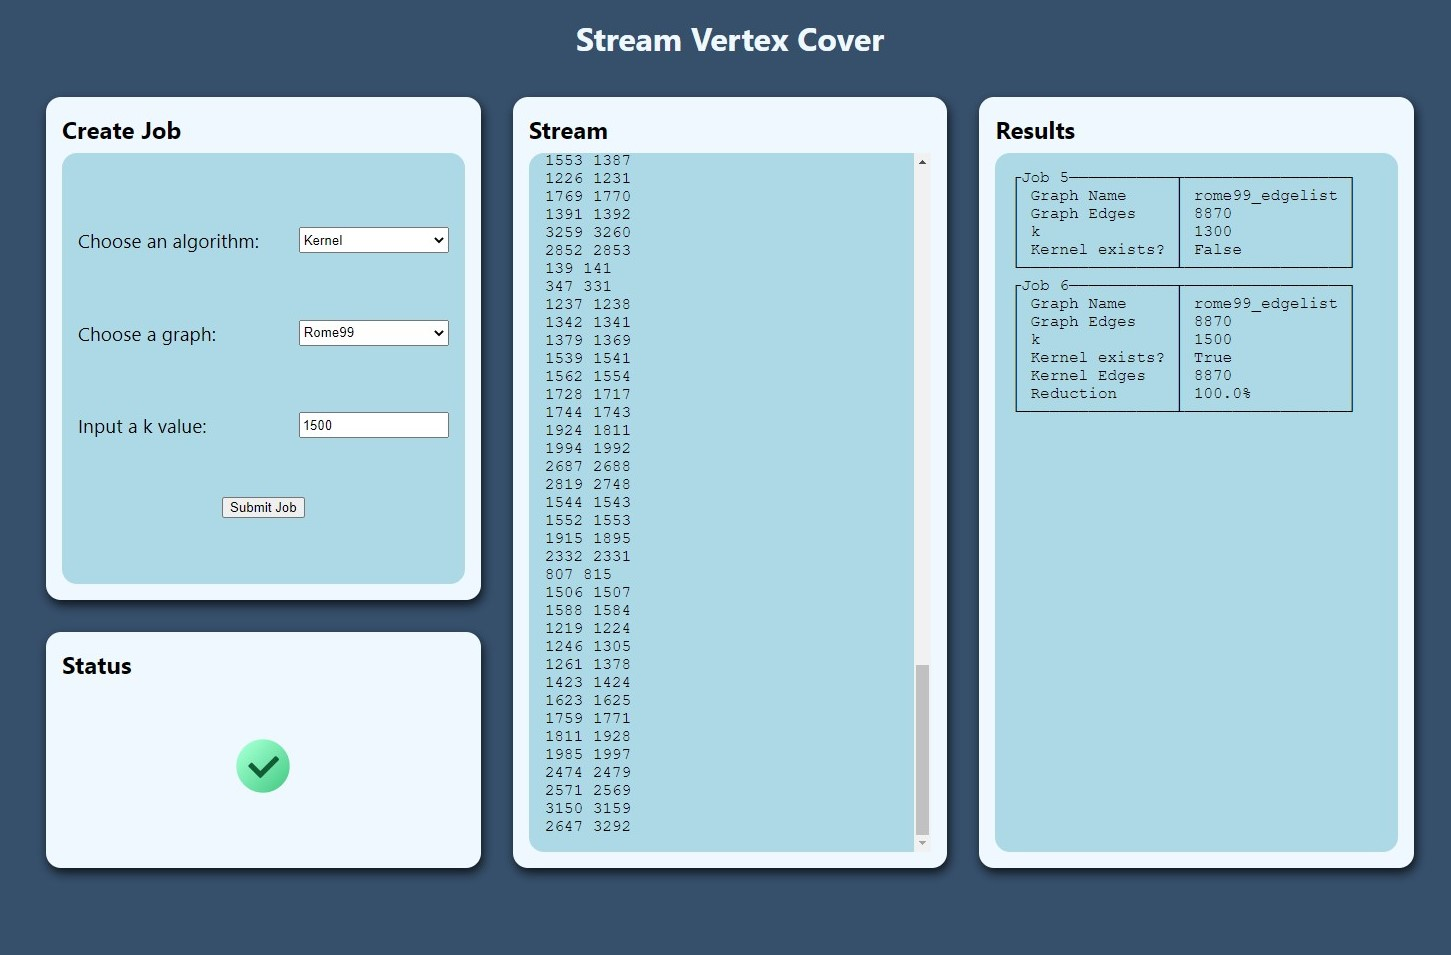
\includegraphics[width=\textwidth]{stream_crop.jpg}
        \end{column}
        \begin{column}{0.3\textwidth}
            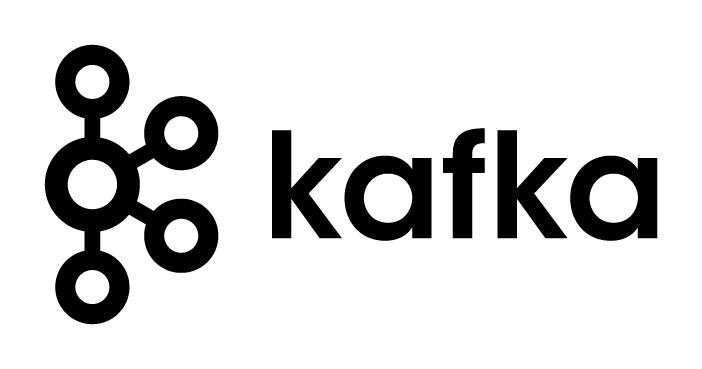
\includegraphics[width=\textwidth]{kafka.png}
        \end{column}
    \end{columns}
\end{frame}

\begin{frame}[standout]
    Thank you - Any questions?
\end{frame}

\end{document}